\noindent
\begin{minipage}[t]{0.26\textwidth}
    \vspace*{0pt}
    \vspace*{215pt}
    
    \noindent
    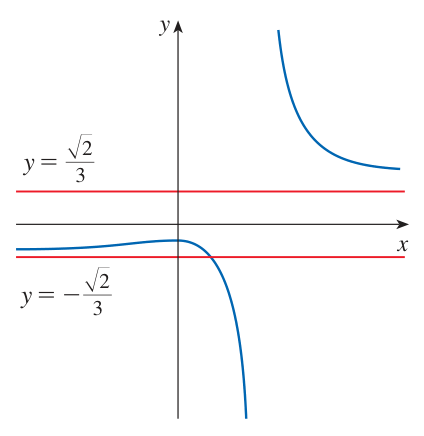
\includegraphics[width=\linewidth]{images/p0166_fig1.png}
    
    \vspace{4pt}
    \noindent{\small\textsf{\textbf{HÌNH 8}}\\[2pt]
    $y = \dfrac{\sqrt{2x^2 + 1}}{3x - 5}$\par}
    
    \vspace{48pt}
    \noindent{\footnotesize\raggedright Ta có thể coi hàm số đã cho có mẫu số bằng $1$.\par}
    
    \vspace{22pt}
    \noindent
    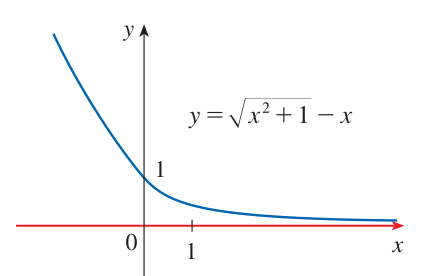
\includegraphics[width=\linewidth]{images/p0166_fig2.png}
    
    \vspace{4pt}
    \noindent{\small\textsf{\textbf{HÌNH 9}}\par}
\end{minipage}%
\hfill
\begin{minipage}[t]{0.71\textwidth}
    \vspace*{0pt}
    \noindent\dots kết quả của các phép tính này bằng cách chỉ ra đồ thị của hàm phân thức đã cho tiệm cận đến đường tiệm cận ngang $y = \frac{3}{5} = 0{,}6$.\hfill{\color{stewartcyan}$\blacksquare$}

    \vspace{1em}
    \noindent\textbf{\textsf{\color{stewartcyan}VÍ DỤ 4}}\hspace{1em}Tìm các đường tiệm cận ngang của đồ thị hàm số
    \[
    f(x) = \frac{\sqrt{2x^2 + 1}}{3x - 5}
    \]

    \noindent\textbf{\textsf{\color{stewartcyan}LỜI GIẢI}}\hspace{1em}Chia cả tử số và mẫu số cho $x$ (là lũy thừa bậc cao nhất của $x$ ở mẫu số) và sử dụng các tính chất của giới hạn, ta có
    \begin{align*}
    \lim_{x \to \infty} \frac{\sqrt{2x^2 + 1}}{3x - 5}
    &= \lim_{x \to \infty} \frac{\dfrac{\sqrt{2x^2 + 1}}{x}}{\dfrac{3x - 5}{x}}
    = \lim_{x \to \infty} \frac{\sqrt{\dfrac{2x^2 + 1}{x^2}}}{\dfrac{3x - 5}{x}}
    \qquad {\color{stewartcyan}(\text{vì } \sqrt{x^2} = x \text{ khi } x > 0)}\\[8pt]
    &= \frac{\lim\limits_{x \to \infty} \sqrt{2 + \dfrac{1}{x^2}}}{\lim\limits_{x \to \infty} \left(3 - \dfrac{5}{x}\right)}
    = \frac{\sqrt{\lim\limits_{x \to \infty} 2 + \lim\limits_{x \to \infty} \dfrac{1}{x^2}}}{\lim\limits_{x \to \infty} 3 - 5 \lim\limits_{x \to \infty} \dfrac{1}{x}}
    = \frac{\sqrt{2 + 0}}{3 - 5 \cdot 0} = \frac{\sqrt{2}}{3}
    \end{align*}

    \noindent Do đó, đường thẳng $y = \sqrt{2}/3$ là một đường tiệm cận ngang của đồ thị hàm số $f$.

    Khi tính giới hạn khi $x \to -\infty$, chúng ta phải nhớ rằng với $x < 0$, ta có $\sqrt{x^2} = |x| = -x$. Vì vậy, khi chia tử số cho $x$, với $x < 0$ ta được
    \[
    \frac{\sqrt{2x^2 + 1}}{x} = \frac{\sqrt{2x^2 + 1}}{-\sqrt{x^2}} = -\sqrt{\frac{2x^2 + 1}{x^2}} = -\sqrt{2 + \frac{1}{x^2}}
    \]

    \noindent Do đó
    \begin{align*}
    \lim_{x \to -\infty} \frac{\sqrt{2x^2 + 1}}{3x - 5}
    &= \lim_{x \to -\infty} \frac{-\sqrt{2 + \dfrac{1}{x^2}}}{3 - \dfrac{5}{x}}
    = -\frac{\sqrt{2 + \lim\limits_{x \to -\infty} \dfrac{1}{x^2}}}{3 - 5 \lim\limits_{x \to -\infty} \dfrac{1}{x}}
    = -\frac{\sqrt{2}}{3}
    \end{align*}

    \noindent Như vậy, đường thẳng $y = -\sqrt{2}/3$ cũng là một đường tiệm cận ngang. Xem Hình~8.\hfill{\color{stewartcyan}$\blacksquare$}

    \vspace{1em}
    \noindent\textbf{\textsf{\color{stewartcyan}VÍ DỤ 5}}\hspace{1em}Tính $\lim\limits_{x \to \infty} \left(\sqrt{x^2 + 1} - x\right)$.

    \vspace{0.2em}
    \noindent\textbf{\textsf{\color{stewartcyan}LỜI GIẢI}}\hspace{1em}Vì cả $\sqrt{x^2 + 1}$ và $x$ đều lớn khi $x$ lớn, nên rất khó để nhận biết điều gì xảy ra với hiệu của chúng, do đó ta dùng đại số để viết lại hàm số. Trước tiên, ta nhân cả tử số và mẫu số với biểu thức căn liên hợp:
    \begin{align*}
    \lim_{x \to \infty} \left(\sqrt{x^2 + 1} - x\right)
    &= \lim_{x \to \infty} \left(\sqrt{x^2 + 1} - x\right) \frac{\sqrt{x^2 + 1} + x}{\sqrt{x^2 + 1} + x}\\[6pt]
    &= \lim_{x \to \infty} \frac{(x^2 + 1) - x^2}{\sqrt{x^2 + 1} + x}
    = \lim_{x \to \infty} \frac{1}{\sqrt{x^2 + 1} + x}
    \end{align*}

    \noindent Để ý rằng mẫu số của biểu thức cuối cùng này ($\sqrt{x^2 + 1} + x$) trở nên rất lớn khi $x \to \infty$ (nó lớn hơn $x$). Do đó
    \[
    \lim_{x \to \infty} \left(\sqrt{x^2 + 1} - x\right) = \lim_{x \to \infty} \frac{1}{\sqrt{x^2 + 1} + x} = 0
    \]

    \noindent Hình~9 minh họa cho kết quả này.\hfill{\color{stewartcyan}$\blacksquare$}
\end{minipage}
